\documentclass[tikz, border = 5pt]{standalone}
\usepackage{tikz}

\usetikzlibrary{arrows.meta}
\usetikzlibrary{shapes.geometric}

\begin{document}

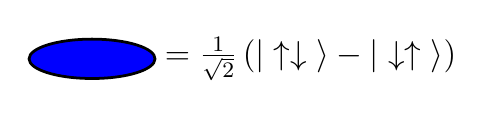
\begin{tikzpicture}[scale = 1.0]

	% dimensions
	\def \a{1}


	% artistic parameters -> check that these are consistent!
	\def \lw{1pt}
	\def \ellength{0.8} % in units of a!
	\def \elheigth{0.25} % in units of a!
	\def \elfillcolor{blue}
	\def \ellinecolor{black}
	\def \ellinewidth{1}
	\def \eltextdistance{0} % in units of r


	\draw[draw=\ellinecolor, fill=\elfillcolor, line width = \ellinewidth] (0, 0) ellipse[x radius = \a*\ellength, y radius = \a*\elheigth];
	
	\pgfmathsetmacro{\X}{\a*(\ellength + \eltextdistance)}

	\node[anchor = west, font = \large] at (\X,0) {$= \frac{1}{\sqrt{2}}\left( \big| \uparrow \downarrow \big\rangle - \big| \downarrow \uparrow \big\rangle \right)$};
	


\end{tikzpicture}
		
\end{document}

